\documentclass{article}
\usepackage{tikz}
\usetikzlibrary{automata,positioning}

\begin{document}

\begin{figure}[h]
    \centering
    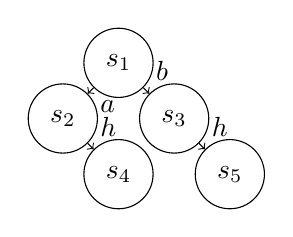
\begin{tikzpicture}[node distance=1cm, auto]
        % States
        \node[state] (s1) {$s_1$};
        \node[state] (s2) [below left of=s1] {$s_2$};
        \node[state] (s3) [below right of=s1] {$s_3$};
        \node[state] (s4) [below right of=s2] {$s_4$};
        \node[state] (s5) [below right of=s3] {$s_5$};

        % Edges
        \path[->] 
            (s1) edge node {$a$} (s2)
            (s1) edge node {$b$} (s3)
            (s2) edge node {$h$} (s4)
            (s3) edge node {$h$} (s5);
    \end{tikzpicture}
    \caption{(a) Initial state machine with states $s_1$, $s_2$, $s_3$, $s_4$, and $s_5$.}
    \label{fig:sample_369_a}
\end{figure}

\begin{figure}[h]
    \centering
    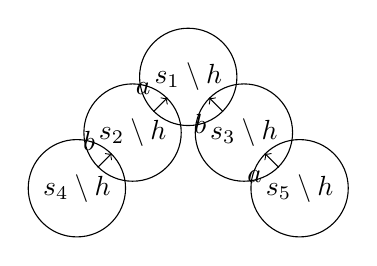
\begin{tikzpicture}[node distance=1cm, auto]
        % States
        \node[state] (s1) {$s_1 \setminus h$};
        \node[state] (s2) [below left of=s1] {$s_2 \setminus h$};
        \node[state] (s3) [below right of=s1] {$s_3 \setminus h$};
        \node[state] (s4) [below left of=s2] {$s_4 \setminus h$};
        \node[state] (s5) [below right of=s3] {$s_5 \setminus h$};

        % Edges
        \path[->] 
            (s1) edge node {$a$} (s2)
            (s1) edge node {$b$} (s3)
            (s2) edge node {$b$} (s4)
            (s3) edge node {$a$} (s5);
    \end{tikzpicture}
    \caption{(b) State machine after removing $h$ from $s_1$, $s_2$, and $s_3$.}
    \label{fig:sample_369_b}
\end{figure}

\begin{figure}[h]
    \centering
    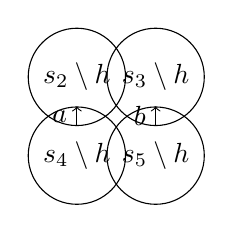
\begin{tikzpicture}[node distance=1cm, auto]
        % States
        \node[state] (s2) {$s_2 \setminus h$};
        \node[state] (s3) [right of=s2] {$s_3 \setminus h$};
        \node[state] (s4) [below of=s2] {$s_4 \setminus h$};
        \node[state] (s5) [below of=s3] {$s_5 \setminus h$};

        % Edges
        \path[->] 
            (s2) edge node {$a$} (s4)
            (s3) edge node {$b$} (s5);
    \end{tikzpicture}
    \caption{(c) State machine after further simplification.}
    \label{fig:sample_369_c}
\end{figure}

\end{document}